% !TeX program = pdfLaTeX
\documentclass[12pt]{article}
\usepackage{amsmath}
\usepackage{graphicx,psfrag,epsf}
\usepackage{enumerate}
\usepackage{natbib}
\usepackage{textcomp}
\usepackage[hyphens]{url} % not crucial - just used below for the URL
\usepackage{hyperref}

%\pdfminorversion=4
% NOTE: To produce blinded version, replace "0" with "1" below.
\newcommand{\blind}{0}

% DON'T change margins - should be 1 inch all around.
\addtolength{\oddsidemargin}{-.5in}%
\addtolength{\evensidemargin}{-.5in}%
\addtolength{\textwidth}{1in}%
\addtolength{\textheight}{1.3in}%
\addtolength{\topmargin}{-.8in}%

%% load any required packages here


% Pandoc syntax highlighting
\usepackage{color}
\usepackage{fancyvrb}
\newcommand{\VerbBar}{|}
\newcommand{\VERB}{\Verb[commandchars=\\\{\}]}
\DefineVerbatimEnvironment{Highlighting}{Verbatim}{commandchars=\\\{\}}
% Add ',fontsize=\small' for more characters per line
\usepackage{framed}
\definecolor{shadecolor}{RGB}{248,248,248}
\newenvironment{Shaded}{\begin{snugshade}}{\end{snugshade}}
\newcommand{\AlertTok}[1]{\textcolor[rgb]{0.94,0.16,0.16}{#1}}
\newcommand{\AnnotationTok}[1]{\textcolor[rgb]{0.56,0.35,0.01}{\textbf{\textit{#1}}}}
\newcommand{\AttributeTok}[1]{\textcolor[rgb]{0.77,0.63,0.00}{#1}}
\newcommand{\BaseNTok}[1]{\textcolor[rgb]{0.00,0.00,0.81}{#1}}
\newcommand{\BuiltInTok}[1]{#1}
\newcommand{\CharTok}[1]{\textcolor[rgb]{0.31,0.60,0.02}{#1}}
\newcommand{\CommentTok}[1]{\textcolor[rgb]{0.56,0.35,0.01}{\textit{#1}}}
\newcommand{\CommentVarTok}[1]{\textcolor[rgb]{0.56,0.35,0.01}{\textbf{\textit{#1}}}}
\newcommand{\ConstantTok}[1]{\textcolor[rgb]{0.00,0.00,0.00}{#1}}
\newcommand{\ControlFlowTok}[1]{\textcolor[rgb]{0.13,0.29,0.53}{\textbf{#1}}}
\newcommand{\DataTypeTok}[1]{\textcolor[rgb]{0.13,0.29,0.53}{#1}}
\newcommand{\DecValTok}[1]{\textcolor[rgb]{0.00,0.00,0.81}{#1}}
\newcommand{\DocumentationTok}[1]{\textcolor[rgb]{0.56,0.35,0.01}{\textbf{\textit{#1}}}}
\newcommand{\ErrorTok}[1]{\textcolor[rgb]{0.64,0.00,0.00}{\textbf{#1}}}
\newcommand{\ExtensionTok}[1]{#1}
\newcommand{\FloatTok}[1]{\textcolor[rgb]{0.00,0.00,0.81}{#1}}
\newcommand{\FunctionTok}[1]{\textcolor[rgb]{0.00,0.00,0.00}{#1}}
\newcommand{\ImportTok}[1]{#1}
\newcommand{\InformationTok}[1]{\textcolor[rgb]{0.56,0.35,0.01}{\textbf{\textit{#1}}}}
\newcommand{\KeywordTok}[1]{\textcolor[rgb]{0.13,0.29,0.53}{\textbf{#1}}}
\newcommand{\NormalTok}[1]{#1}
\newcommand{\OperatorTok}[1]{\textcolor[rgb]{0.81,0.36,0.00}{\textbf{#1}}}
\newcommand{\OtherTok}[1]{\textcolor[rgb]{0.56,0.35,0.01}{#1}}
\newcommand{\PreprocessorTok}[1]{\textcolor[rgb]{0.56,0.35,0.01}{\textit{#1}}}
\newcommand{\RegionMarkerTok}[1]{#1}
\newcommand{\SpecialCharTok}[1]{\textcolor[rgb]{0.00,0.00,0.00}{#1}}
\newcommand{\SpecialStringTok}[1]{\textcolor[rgb]{0.31,0.60,0.02}{#1}}
\newcommand{\StringTok}[1]{\textcolor[rgb]{0.31,0.60,0.02}{#1}}
\newcommand{\VariableTok}[1]{\textcolor[rgb]{0.00,0.00,0.00}{#1}}
\newcommand{\VerbatimStringTok}[1]{\textcolor[rgb]{0.31,0.60,0.02}{#1}}
\newcommand{\WarningTok}[1]{\textcolor[rgb]{0.56,0.35,0.01}{\textbf{\textit{#1}}}}

% tightlist command for lists without linebreak
\providecommand{\tightlist}{%
  \setlength{\itemsep}{0pt}\setlength{\parskip}{0pt}}

% From pandoc table feature
\usepackage{longtable,booktabs,array}
\usepackage{calc} % for calculating minipage widths
% Correct order of tables after \paragraph or \subparagraph
\usepackage{etoolbox}
\makeatletter
\patchcmd\longtable{\par}{\if@noskipsec\mbox{}\fi\par}{}{}
\makeatother
% Allow footnotes in longtable head/foot
\IfFileExists{footnotehyper.sty}{\usepackage{footnotehyper}}{\usepackage{footnote}}
\makesavenoteenv{longtable}

% Pandoc citation processing
\newlength{\cslhangindent}
\setlength{\cslhangindent}{1.5em}
\newlength{\csllabelwidth}
\setlength{\csllabelwidth}{3em}
\newlength{\cslentryspacingunit} % times entry-spacing
\setlength{\cslentryspacingunit}{\parskip}
% for Pandoc 2.8 to 2.10.1
\newenvironment{cslreferences}%
  {}%
  {\par}
% For Pandoc 2.11+
\newenvironment{CSLReferences}[2] % #1 hanging-ident, #2 entry spacing
 {% don't indent paragraphs
  \setlength{\parindent}{0pt}
  % turn on hanging indent if param 1 is 1
  \ifodd #1
  \let\oldpar\par
  \def\par{\hangindent=\cslhangindent\oldpar}
  \fi
  % set entry spacing
  \setlength{\parskip}{#2\cslentryspacingunit}
 }%
 {}
\usepackage{calc}
\newcommand{\CSLBlock}[1]{#1\hfill\break}
\newcommand{\CSLLeftMargin}[1]{\parbox[t]{\csllabelwidth}{#1}}
\newcommand{\CSLRightInline}[1]{\parbox[t]{\linewidth - \csllabelwidth}{#1}\break}
\newcommand{\CSLIndent}[1]{\hspace{\cslhangindent}#1}

\usepackage{booktabs}
\usepackage{longtable}
\usepackage{array}
\usepackage{multirow}
\usepackage{wrapfig}
\usepackage{float}
\usepackage{colortbl}
\usepackage{pdflscape}
\usepackage{tabu}
\usepackage{threeparttable}
\usepackage{threeparttablex}
\usepackage[normalem]{ulem}
\usepackage{makecell}
\usepackage{xcolor}

\begin{document}


\def\spacingset#1{\renewcommand{\baselinestretch}%
{#1}\small\normalsize} \spacingset{1}


%%%%%%%%%%%%%%%%%%%%%%%%%%%%%%%%%%%%%%%%%%%%%%%%%%%%%%%%%%%%%%%%%%%%%%%%%%%%%%

\if0\blind
{
  \title{\bf Three (Groups of) Blind Mice. Familial Clusters of Cataract Development in Irradiated Mice}

  \author{
        Alyssa Allsop and Amira Burns \\
    Department of Statistics, Colorado State University\\
      }
  \maketitle
} \fi

\if1\blind
{
  \bigskip
  \bigskip
  \bigskip
  \begin{center}
    {\LARGE\bf Three (Groups of) Blind Mice. Familial Clusters of Cataract Development in Irradiated Mice}
  \end{center}
  \medskip
} \fi

\bigskip
\begin{abstract}
Astronauts traveling outside Earth's protective magnetic field are exposed to radiation with potentially serious side effects - one such effect is development of cataracts. Studying cataracts caused by radiation is complicated by genetic predisposition or resistance to cataract development. This study exposed mice bred in genetic families to specific types of radiation to examine familial clustering of cataracts. A mixed effects logistic regression model was fit to the data; the final model included parameters for sex, treatment group, sex by treatment group interaction, and a random intercept for family. Family was shown to be an important source of variation in predicting cataract development. Male sex was associated with differences in cataract development among treatment groups, while evidence showed little association between female sex and cataract development across among treatment groups. Males were more likely to develop severe cataracts than females across all three treatment groups.
\end{abstract}

\noindent%
{\it Keywords:} Hierarchical modeling, Logistic regression, Bayesian analysis
\vfill

\newpage
\spacingset{1.45} % DON'T change the spacing!

\section{Introduction}
\label{sec:intro}

Little is known about the effects of high atomic number and energy (HZE) radiation, a main component of space radiation to which exposure is unavoidable beyond Earth's magnetic field. In contrast, extensive research has shown that exposure to high doses of gamma radiation leads to acute radiation sickness. Adverse effects from radiation may also be attributable to other factors, including genetics; several different cancers have been observed to cluster in mice families \citep{mice2017}. This analysis examines potential genetic susceptibility to cataract development in the presence of radiation treatment.\\
<<<<<<< HEAD
The experiment included 1820 unique mice from 48 unique families, bred over several generations to create a genetically heterogeneous sample. Individuals were randomly assigned, with equal family weight, to one of three radiation treatment groups: HZE irradiation, gamma irradiation, and non-irradiated control. Mice in both irradiated groups were exposed to radiation at 7-12 weeks of age, and all mice were monitored weekly until 800 days of age. This analysis used a simplified version of the data that contained final observations for the 1169 mice from 47 unique families that survived at least 552 days. Family size ranged \([11, 48]\), with median family size \(= 24\).\\
=======
The experiment included 1820 unique mice from 48 unique families, bred over several generations to create a genetically heterogeneous sample. Individuals were randomly assigned, with equal family weight, to one of three radiation treatment groups: HZE irradiation, gamma irradiation, and non-irradiated control. Mice in both irradiated groups were exposed to radiation at 7-12 weeks of age, and all mice were monitored weekly until 800 days of age. This analysis used a simplified version of the data set containing observations at death for the 1169 mice from 47 unique families that survived at least 552 days. Family size ranged \([11, 48]\), with median family size \(= 24\).\\
>>>>>>> b3193c3af4ca0cb4ddc5be2138ed7ebea9613211

\begin{wraptable}{r}{0pt}
\centering
\begin{tabular}{lrrrrr}
  \toprule
\multicolumn{1}{c}{ } & \multicolumn{4}{c}{Cataract Score} & \multicolumn{1}{c}{ } \\
\cmidrule(l{3pt}r{3pt}){2-5}
Treatment & 1 & 2 & 3 & 4 & Total \\ 
  \midrule
Unirradiated & 438 &  45 &  11 &   2 & 496 \\ 
  Gamma & 214 &  53 &   6 &   4 & 277 \\ 
  HZE & 281 & 107 &   6 &   2 & 396 \\ 
   \bottomrule
\end{tabular}
\caption{Counts of score by treatment group} 
\label{tab:gtab}
\end{wraptable}

<<<<<<< HEAD
Due to small group sizes (Table \ref{tab:gtab}), the response was converted from a discrete ordinal variable (levels = \([1, 2, 3, 4]\)) matching ocular changes in the eye to a binary variable where score \(\ge 2\) indicated presence of cataracts. Both the main experimental factor, Treatment, and the single random effect, genetic Family, were central to the experimental design and of primary research interest; consequently, both variables were included in all models considered. Additional covariates under consideration were sex, coat color, weight in grams, body condition score (BCS), age in days, and presence of three cancers: myeloid leukemia, harderian tumors, and pre-T lymphoma.
=======
Due to small group sizes (Table \ref{tab:gtab}), the response was converted from a discrete ordinal variable (levels = {[}1, 2, 3, 4{]}) matching ocular changes in the eye to a binary variable where score \(\ge\) 2 indicated presence of cataracts. Both the main experimental factor, Treatment, and the single random effect, genetic Family, were central to the experimental design and of primary research interest; consequently, both variables were included in all models considered. Additional covariates under consideration were sex, coat color, weight in grams, body condition score (BCS), age in days, and presence of three cancers: myeloid leukemia, harderian tumors, and pre-T lymphoma.
>>>>>>> b3193c3af4ca0cb4ddc5be2138ed7ebea9613211

\section{Summary Statistics}
\label{sec:sumstats}

Exploratory data analysis focused on assessing cataracts status in terms of treatment group, and potential associations between covariates and the response. Tables and graphs (available in Appendix \ref{sec:appeda}) were created to investigate any empirical associations between coviarates and either treatment group or cataract status. Further examination of potential covariates revealed distinct patterns of cataracts status between male and female mice, as shown in Figure \ref{fig:bareda}.\\

\begin{figure}[H]

{\centering 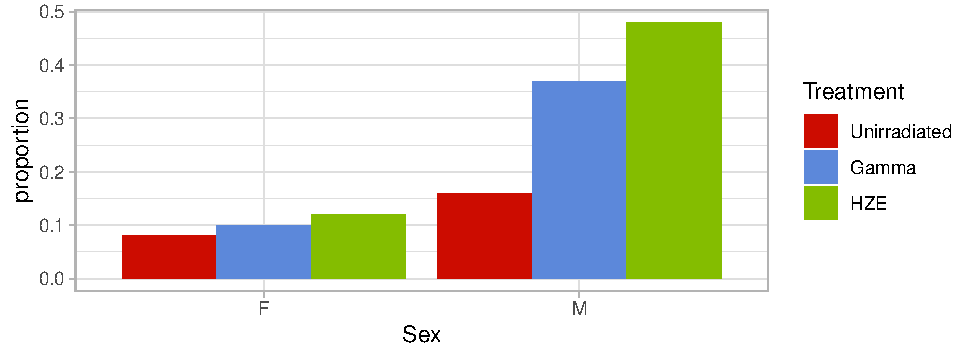
\includegraphics{bookdown_report_files/figure-latex/bareda-1} 

}

\caption{Sample proportions with cataracts by sex, treatment group}\label{fig:bareda}
\end{figure}

Empirical assessment of the effect of family across treatment group did not display apparent clustering where scores were higher across treatment groups in some families. Figure \ref{fig:lineeda} did reveal some distinct patterns across families and treatment groups; for example, the Gamma treatment group appeared to have either the highest group score per family, or the lowest group score per family.\\

\begin{figure}[H]

{\centering 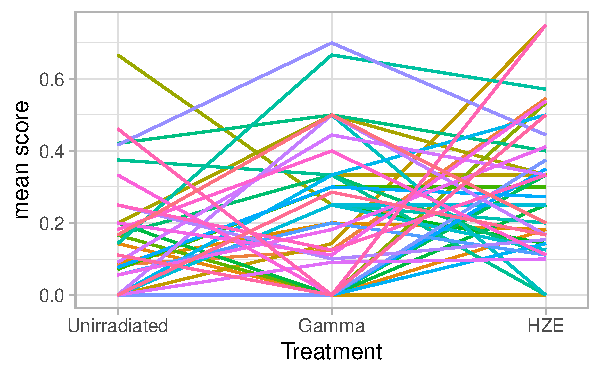
\includegraphics{bookdown_report_files/figure-latex/lineeda-1} 

}

\caption{Mean family cataract score by treatment group}\label{fig:lineeda}
\end{figure}

\section{Statistical Methods}
\label{sec:methods}

Hierarchical logistic regression was selected as the primary analytic method, due to the binary response and random effect of interest to the research question. Various models were fit and assessed using Aikike's Information Criterion (AIC); see Appendix \ref{sec:glmms} for the full list of models examined. The final model can be written as:\\
\begin{equation}
\begin{aligned}
Y_{ij} \sim &Bernoulli(p) \\
log(\frac{p}{1-p}) = &\ \beta_0\ +\beta_1*Gamma_i\ + \beta_2*HZE_i\ + \beta_3*M_i\ + \\ &\beta_4*Gamma_i*M_i\ + \beta_5*HZE_i*M_i\ +\ [v_{j} + \epsilon_{ij}] \\
&i = 1, ..., 1169\ \mbox{ mice}\ \ \ \ j = 1,...,47\ \ \mbox{ families}
\end{aligned}
\label{eq:glmm}
\end{equation}\\
where \(M_i\) is an indicator for males, \(v_{j}\) is the variance of the random intercept for Family \(j\), and \(\epsilon_{ij}\) is the residual variance. Model assumptions of Normally-distributed random effects and lack of overdispersion were verified in Appendix \ref{sec:glmmd}.

A complementary Bayesian model with non-informative priors was fit to obtain probability distributions of the parameters from the final model, as well as test the estimates' robustness to alternative approaches \citep{BDA}. This model can be written as:\\
\begin{equation}
\begin{aligned}
Y_{ij} \sim &Bernoulli(p)\\
log(\frac{p}{1-p}) = &\ \beta_0*Control_i*F_i\ +\beta_1*Gamma_i*F_i\ + \beta_2*HZE_i*F_i\ + \\ &\beta_3*Control_i*M_i\ +\beta_4*Gamma*M\ + \beta_5*HZE*M\ + \\
&v_{j} + \epsilon_{ij}\\
&i = 1, ..., 1169\ \mbox{ mice}\ \ \ \ j = 1,...,47\ \ \mbox{ families, and} \\
v_j \sim\ &N(0, \tau)
\\
&\mbox{ with non-informative priors:}\\
\beta_0 &\sim N(0, 0.001)\ \ \ \ \beta_1 \sim N(0, 0.001)\ \ \ \ \beta_2 \sim N(0, 0.001)\\
\beta_3 &\sim N(0, 0.001)\ \ \ \ \beta_4 \sim N(0, 0.001)\ \ \ \ \beta_5 \sim N(0, 0.001)\\
v_i &\sim N(0, \sigma^2)\\
\tau &\sim Gamma(0.001, 0.001) \mbox{ where}\ \sigma^2 = 1/\tau 
\end{aligned}
\label{eq:bayes}
\end{equation}

Model \eqref{eq:bayes} was run through a Gibbs sampler Markov Chain Monte Carlo (MCMC) algorithm in the `rjags' package \citep{R-rjags} to approximate the posterior distributions of the estimates of all fixed effects and the variance of the random effect. 3 chains of 60000 total iterations with a 10000-iteration burn-in period; starting values were obtained from the estimates generated by Model \eqref{eq:glmm}, with noise added to avoid false convergence. Full model diagnostics may be accessed in Appendix \ref{sec:bayesd}.

\begin{table}[H]
\centering
\begin{tabular}{rrrrrr}
  \toprule
 & GLMM Est & MCMC Mode & MCMC SD & HPD Lower & HPD Upper \\ 
  \midrule
b\_0 & -2.70 & -2.68 & 0.27 & -3.25 & -2.20 \\ 
  b\_1 & 0.21 & 0.09 & 0.38 & -0.53 & 0.95 \\ 
  b\_2 & 0.50 & 0.49 & 0.33 & -0.14 & 1.15 \\ 
  b\_3 & 0.89 & 0.90 & 0.30 & 0.31 & 1.50 \\ 
  b\_4 & 0.97 & 1.09 & 0.46 & 0.08 & 1.88 \\ 
  b\_5 & 1.21 & 1.27 & 0.41 & 0.40 & 2.00 \\ 
  sigma\verb|^|2 & 0.40 & 0.32 & 0.18 & 0.15 & 0.81 \\ 
   \bottomrule
\end{tabular}
\caption{Final model parameter estimates} 
\label{tab:est_tab}
\end{table}

Results from Model \eqref{eq:glmm} and Model \eqref{eq:bayes} were congruent, as shown in Table @ref(tab:est\_tab). The 95\% highest posterior density (HPD) credible intervals from Model \eqref{eq:bayes} offer the advantage of concluding 95\% confidence that estimates for each parameter lie within those bounds.

\section{Limitations and Alternatives}
\label{sec:limits}

Logistic regression assumes linearity of \(log(\frac{p}{1-p})\) \citep{BMLR2021}.
Limitations include lack of robust diagnostic assessment of GLMMs \citep{CDA}.
Presence of competing risks in the experimental design obscure the presence of family clusters of cataracts. Simplifying the dataset by instituting a cutoff age attempts to address this limitation, but the issue persists even after excluding individuals deceased before Age = 552.

\section{Results}
\label{sec:results}

The final probability for developing cataracts can be written as:\\
\begin{equation}
\begin{aligned}
p_{ij} = &0.063 + v_j + 0.55*Gamma_i + 0.623*HZE_i + \\
&0.708*Male_i + 0.726*Gamma_i*Male_i + 0.770*HZE_i*Male_i
\end{aligned}
\label{eq:probs}
\end{equation}

Comparisons of different groups across Sex and Treatment were assessed on Model \eqref{eq:glmm} using the \texttt{emmeans} package \citep{R-emmeans}. Figure \ref{fig:contr} shows of the probability of developing cataracts for each combination of sex by treatment group. Differences between both sex and treatment group were clearly visible, notably the differences between treatment group within gender.

\begin{figure}[H]

{\centering 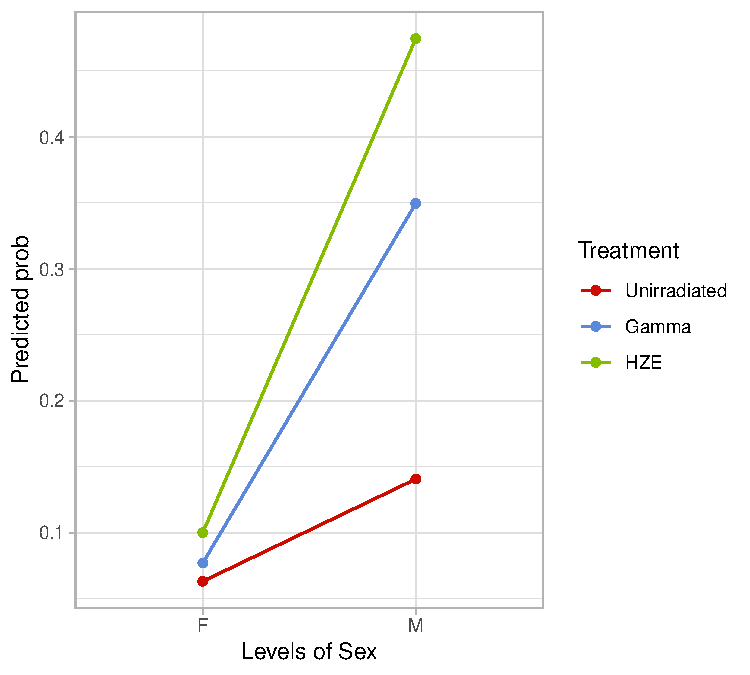
\includegraphics{bookdown_report_files/figure-latex/contr-1} 

}

\caption{Predicted probability of cataracts by sex, treatment group}\label{fig:contr}
\end{figure}

Figure \ref{fig:RR} shows the relative risk of cataract development for all group comparisons in Model \eqref{eq:glmm}. Within females, all relative risks between treatment groups resulted in confidence intervals containing the possibility of no increased risk from exposure. Within males, conversely, all three comparisons between treatment groups showed strong evidence for increased risk with exposure. The largest difference was observed among Males between the HZE group and the control group.\\

\begin{figure}[H]

{\centering 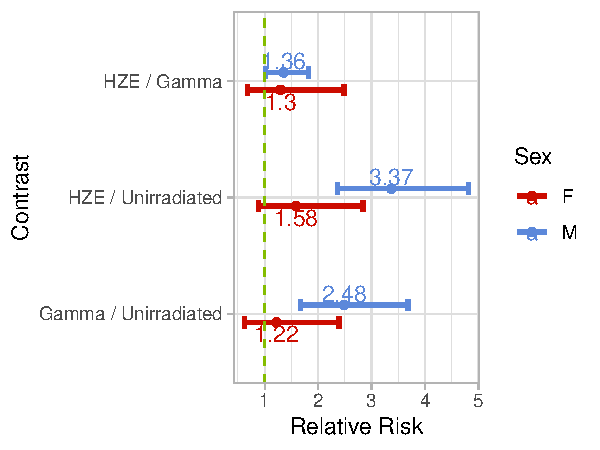
\includegraphics[width=0.5\linewidth]{bookdown_report_files/figure-latex/RR-1} 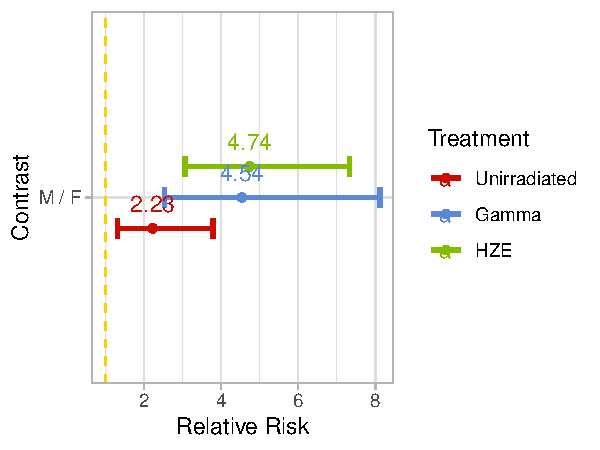
\includegraphics[width=0.5\linewidth]{bookdown_report_files/figure-latex/RR-2} 

}

\caption{Relative risk of cataract development between all group combinations}\label{fig:RR}
\end{figure}

<<<<<<< HEAD
Between sex, a greater relative risk of cataract development was observed for males than females within all treatment groups, although variability between treatment group remained salient. Males had a 4.74 and 4.54 times greater risk of developing severe cataracts than females in the HZE and Gamma groups respectively, compared to only 2.23 times greater risk within the control group.
=======
Figure \ref{fig:RR} shows the relative risk of cataract development for all groups in Model \eqref{eq:glmm}. From the plot on the left we see that mice in the HZE group had a higher risk of developing severe cataracts than both the gamma and control groups. Males in the HZE group had 1.36 times greater risk than males in the gamma group. The biggest difference is seen in the HZE group compared to the unirradiated control group for males. Males in HZE had 3.37 times greater risk than males in the control group. On the right, it is made clear that males have a much higher risk of developing cataracts than females. In the HZE group, males have a 4.74 times higher risk of developing severe cataracts than females and in the gamma group it is a 4.54 times higher risk.

Fix this plot!
>>>>>>> b3193c3af4ca0cb4ddc5be2138ed7ebea9613211

Visualizing random effect by family:\\

\begin{figure}[H]

{\centering 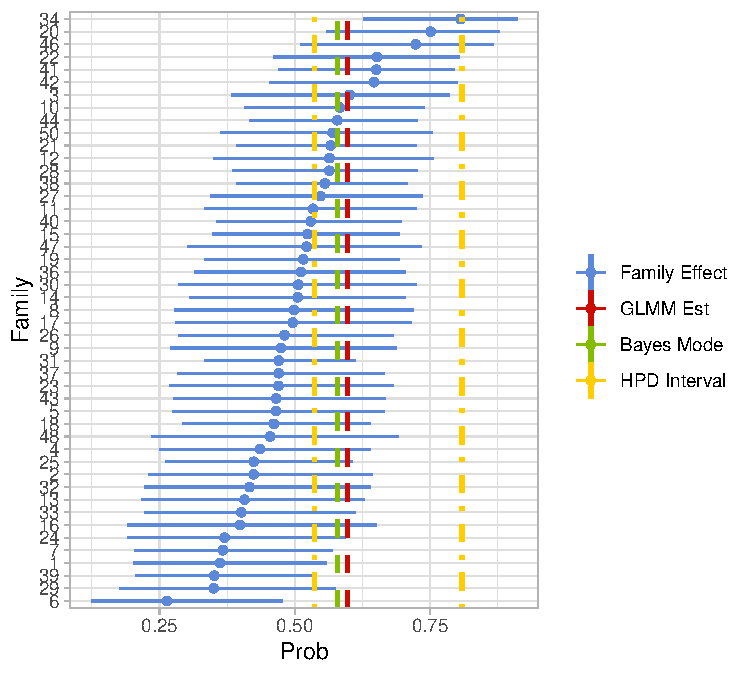
\includegraphics{bookdown_report_files/figure-latex/re-1} 

}

\caption{Estimated random probability of developing cataracts by family}\label{fig:re}
\end{figure}

<<<<<<< HEAD
Figure \ref{fig:re} visualizes the estimated variability of developing cataracts by family on the probability scale, along with confidence intervals. The vertical lines plot the GLMM estimated variance from Model \eqref{eq:glmm} and the MCMC mode and HPD interval for \(\sigma^2\) from Model \eqref{eq:bayes}. The dispersion on the tails of the probability scale indicate plausible genetic predisposition or resistance to cataract development.
=======
Figure \ref{fig:re} visualizes the estimated probability of developing cataracts for each family in the dataset, along with their confidence intervals. The vertical lines plot the GLMM estimated variance from Model \eqref{eq:glmm} and the MCMC mode and HPD interval for \(\sigma^2\) from Model \eqref{eq:bayes}. Many of the probabilities shown are close to 0.5, with small numbers of families at the top and bottom of the graph that indicate some respective genetic predisposition or resistance to cataract development. \textbf{from the comments on our presentation it seemed like Ann thought we shouldn't compare these to 0.5. Not sure how to interpret it otherwise though}
>>>>>>> b3193c3af4ca0cb4ddc5be2138ed7ebea9613211

\section{Conclusions}
\label{sec:conc}

<<<<<<< HEAD
Females faced lower probability of developing cataracts than males across all treatment groups, and the association of treatment group with cataract status was not apparent for female mice in this data set. Males, on the other hand, had a higher probability of developing cataracts than females across all treatment groups, and the differences of cataract development between treatment groups was of clinical importance.
=======
\textbf{Turn this into a nice paragraph or two; add quantitative info from results to back these up, or keep it general?}
**alyssa's thoughts: I think a table would be nice comparing males and females probabilities, but would it fit? and would it be redundant of the line chart showing probabilities among groups and sexes? I don't know if listing out all the numbers of probabilities would be good in sentence form.*

Females in general face less probability of developing cataracts than males, across all treatment groups. We could argue that the effect of treatment group is not of clinical significance for female mice in this dataset. As you can see, the probability of developing cataracts is quite low for all 3 treatment groups. Males, on the other hand, have a higher probability of developing cataracts than females across all treatment groups. For males, the differences of development of cataracts across treatment groups is of clinical importance.
>>>>>>> b3193c3af4ca0cb4ddc5be2138ed7ebea9613211

\section{Author's Statements}
\label{sec:auth}

Both authors contributed to statistical analysis and writing for this report. Both authors read and approved the final report. Both authors contributed equally to introduction, exploratory data analysis, summary statistics, and results. Alyssa Allsop served as the primary statistician on fitting Frequentist models; Amira Burns served as the primary statistician on fitting the Bayesian model.

\newpage

<<<<<<< HEAD
\hypertarget{references}{%
\section{References}\label{references}}

\hypertarget{refs}{}
\begin{CSLReferences}{0}{0}
\end{CSLReferences}

=======
>>>>>>> b3193c3af4ca0cb4ddc5be2138ed7ebea9613211
\appendix

\section{Appendix}

\hypertarget{additional-exploratory-data-analysis}{%
\subsection{Additional Exploratory Data Analysis}\label{additional-exploratory-data-analysis}}

\label{sec:appeda}

\begin{figure}[H]

{\centering 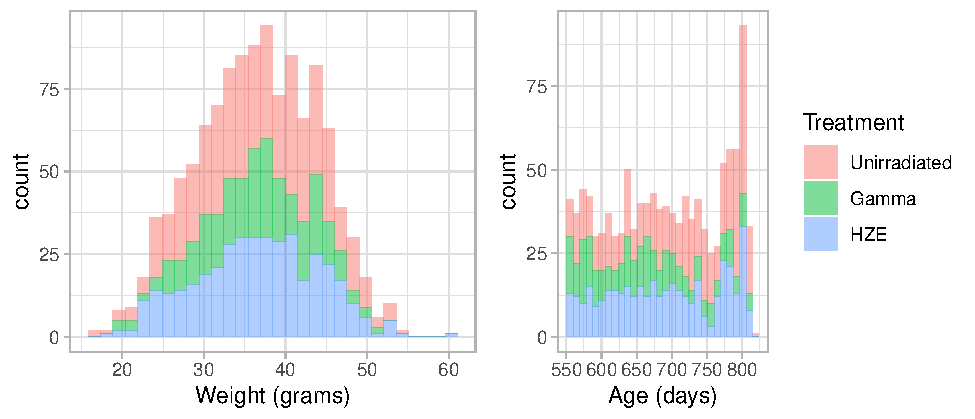
\includegraphics[width=0.42\linewidth]{bookdown_report_files/figure-latex/eda-1} 

}

\caption{Histograms of contiguous covariates by treatment group}\label{fig:eda-1}
\end{figure}
\begin{figure}[H]

{\centering 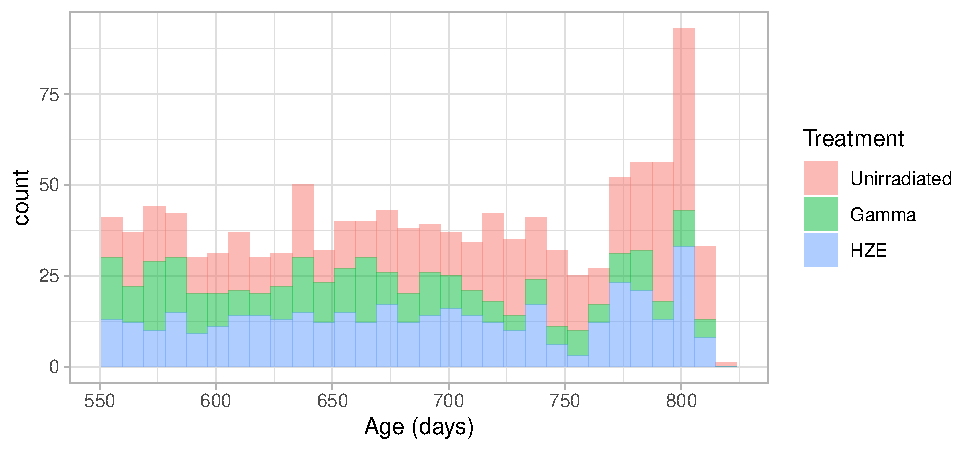
\includegraphics[width=0.42\linewidth]{bookdown_report_files/figure-latex/eda-2} 

}

\caption{Histograms of contiguous covariates by treatment group}\label{fig:eda-2}
\end{figure}

\begin{table}[!h]
\centering
\begin{tabular}{lllr}
  \toprule
MyeloidLeukemia & HarderianTumor & PreTLymphoma & n \\ 
  \midrule
0 & bilateral & 0 &  39 \\ 
  0 & none & 0 & 954 \\ 
  0 & none & 1 &   6 \\ 
  0 & unilateral & 0 & 134 \\ 
  0 & unilateral & 1 &   1 \\ 
  1 & none & 0 &  30 \\ 
  1 & none & 1 &   1 \\ 
  1 & unilateral & 0 &   4 \\ 
   \bottomrule
\end{tabular}
\caption{Counts of cancer status} 
\end{table}

\begin{figure}[H]

{\centering 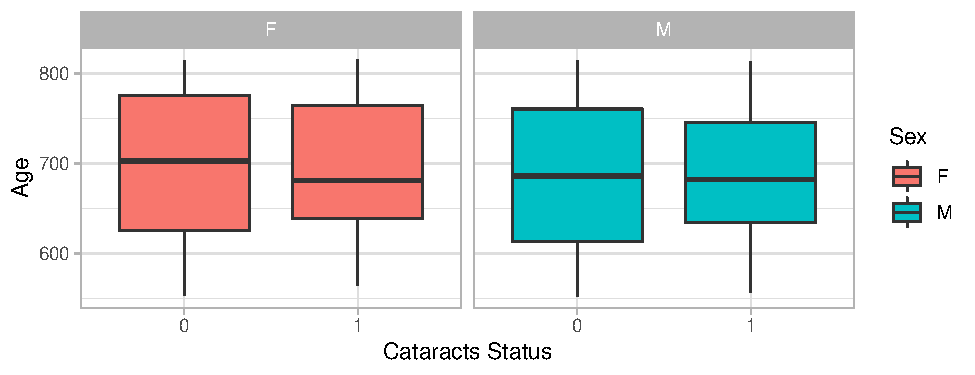
\includegraphics[width=0.5\linewidth]{bookdown_report_files/figure-latex/scage-1} 

}

\caption{Boxplot of Age, cataracts status by sex and treatment}\label{fig:scage-1}
\end{figure}
\begin{figure}[H]

{\centering 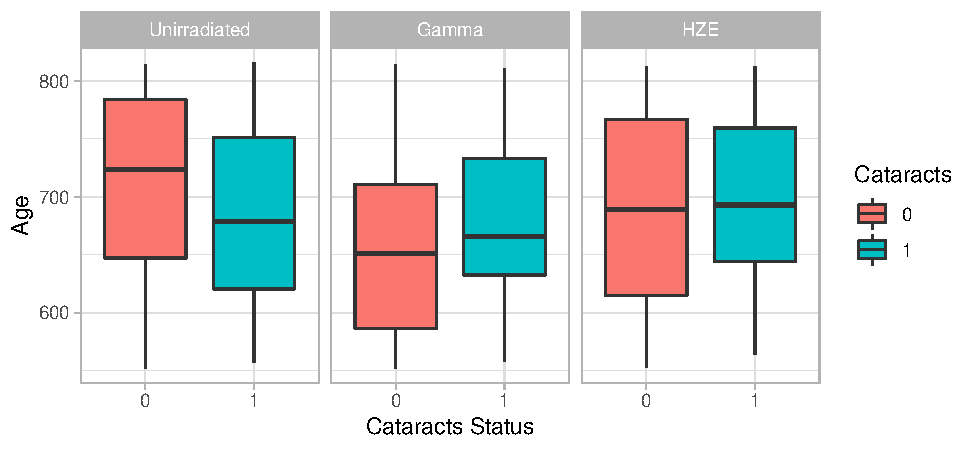
\includegraphics[width=0.5\linewidth]{bookdown_report_files/figure-latex/scage-2} 

}

\caption{Boxplot of Age, cataracts status by sex and treatment}\label{fig:scage-2}
\end{figure}

\begin{figure}[H]

{\centering 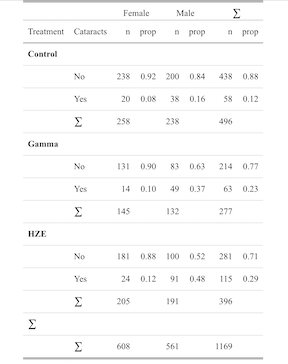
\includegraphics[width=0.5\linewidth]{ct_prop} 

}

\caption{Table of counts and proportions by sex, treatment group, cataracts status}\label{fig:ctprop}
\end{figure}

\hypertarget{model-selection}{%
\subsection{Model Selection}\label{model-selection}}

\label{sec:glmms}

AIC was used as the primary model selection criteria because it can be used to compare non-nested models. This feature was of particular importance when assessing models with a random effect against a model with only fixed effects.

\begin{table}[!h]
\centering
\begin{tabular}{ll}
  \toprule
Model & AIC \\ 
  \midrule
Final Model & 1017.98 \\ 
  Full Mixed Model & 1038.9 \\ 
  Fixed Effects Model & 1040.3 \\ 
  Mixed Model with no Interaction & 1023.19 \\ 
  Base Model & 1123.57 \\ 
   \bottomrule
\end{tabular}
\caption{Model selection via AIC comparision} 
\end{table}

\hypertarget{glm-model-diagnostics}{%
\subsection{GLM Model Diagnostics}\label{glm-model-diagnostics}}

\label{sec:glmmd}

\begin{figure}[H]

{\centering 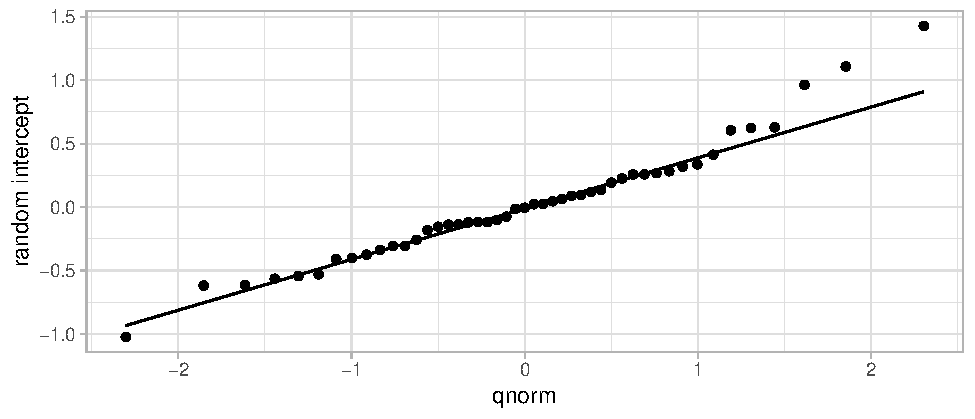
\includegraphics{bookdown_report_files/figure-latex/qq-1} 

}

\caption{QQ-plot of random effect on intercept}\label{fig:qq}
\end{figure}

Assumptions for fitting this model were: the random effects came from a normal distribution; the chosen link function was appropriate; and estimation of variance was not over-dispersed. These assumptions were verified. Quantiles of the random effect were compared with the quantiles of a normal distribution and looked approximately normal in Figure \ref{fig:qq}. The chosen logit link function was appropriate because the response used was binary. The ratio of the chi square statistic to the residual degrees of freedom was 0.89; a value \(\le\) 1 indicates no over-dispersion.

\hypertarget{bayesian-model-diagnostics}{%
\subsection{Bayesian Model Diagnostics}\label{bayesian-model-diagnostics}}

\label{sec:bayesd}

\hypertarget{source-code}{%
\subsection{Source Code}\label{source-code}}

\begin{Shaded}
\begin{Highlighting}[]
<<<<<<< HEAD
\NormalTok{knitr}\SpecialCharTok{::}\NormalTok{opts\_chunk}\SpecialCharTok{$}\FunctionTok{set}\NormalTok{(}\AttributeTok{fig.height=}\DecValTok{3}\NormalTok{, }\AttributeTok{fig.pos =} \StringTok{\textquotesingle{}H\textquotesingle{}}\NormalTok{, }\AttributeTok{fig.align =} \StringTok{\textquotesingle{}center\textquotesingle{}}\NormalTok{,}
=======
\NormalTok{knitr}\SpecialCharTok{::}\NormalTok{opts\_chunk}\SpecialCharTok{$}\FunctionTok{set}\NormalTok{(}\AttributeTok{fig.height=}\FloatTok{2.5}\NormalTok{, }\AttributeTok{fig.pos =} \StringTok{\textquotesingle{}H\textquotesingle{}}\NormalTok{, }\AttributeTok{fig.align =} \StringTok{\textquotesingle{}center\textquotesingle{}}\NormalTok{,}
>>>>>>> b3193c3af4ca0cb4ddc5be2138ed7ebea9613211
                      \AttributeTok{echo=}\ConstantTok{FALSE}\NormalTok{, }\AttributeTok{warning=}\ConstantTok{FALSE}\NormalTok{, }\AttributeTok{message=}\ConstantTok{FALSE}\NormalTok{) }

\FunctionTok{library}\NormalTok{(readxl)}
\FunctionTok{library}\NormalTok{(tidyverse)}
\FunctionTok{library}\NormalTok{(DescTools)}
\FunctionTok{library}\NormalTok{(lme4)}
\FunctionTok{library}\NormalTok{(broom.mixed)}
\FunctionTok{library}\NormalTok{(kableExtra)}
\FunctionTok{library}\NormalTok{(xtable)}
\FunctionTok{library}\NormalTok{(emmeans)}
\FunctionTok{library}\NormalTok{(ggsci)}
\FunctionTok{library}\NormalTok{(sjPlot)}
\FunctionTok{library}\NormalTok{(coda)}
\FunctionTok{library}\NormalTok{(rjags)}
\FunctionTok{library}\NormalTok{(R2jags)}
\FunctionTok{library}\NormalTok{(superdiag)}
\FunctionTok{library}\NormalTok{(mcmcplots)}
\FunctionTok{library}\NormalTok{(ggmcmc)}
\FunctionTok{library}\NormalTok{(gridExtra)}
\NormalTok{cats }\OtherTok{\textless{}{-}} \FunctionTok{read\_excel}\NormalTok{(}\AttributeTok{path =} \StringTok{"GRSD.cataract.xlsx"}\NormalTok{, }\AttributeTok{sheet =} \StringTok{"Sheet1"}\NormalTok{)}
\CommentTok{\# remove spaces from column and value names}
\FunctionTok{names}\NormalTok{(cats) }\OtherTok{\textless{}{-}} \FunctionTok{str\_replace\_all}\NormalTok{(}\FunctionTok{names}\NormalTok{(cats), }\StringTok{" "}\NormalTok{, }\StringTok{"\_"}\NormalTok{)}
\NormalTok{cats }\OtherTok{\textless{}{-}}\NormalTok{ cats }\SpecialCharTok{\%\textgreater{}\%}
  \FunctionTok{mutate}\NormalTok{(}\AttributeTok{CoatColor =} \FunctionTok{str\_replace\_all}\NormalTok{(coat\_color, }\StringTok{" "}\NormalTok{, }\StringTok{"\_"}\NormalTok{))}

\CommentTok{\# turn categorical vars into factor}
\NormalTok{cats }\OtherTok{\textless{}{-}}\NormalTok{ cats }\SpecialCharTok{\%\textgreater{}\%}
  \FunctionTok{rename}\NormalTok{(}\AttributeTok{Age =} \StringTok{\textasciigrave{}}\AttributeTok{age\_(days)}\StringTok{\textasciigrave{}}\NormalTok{,}
         \AttributeTok{Weight =}\NormalTok{ weight,}
         \AttributeTok{Animal =}\NormalTok{ animal) }\SpecialCharTok{\%\textgreater{}\%}
  \FunctionTok{mutate}\NormalTok{(}\AttributeTok{Sex =} \FunctionTok{as.factor}\NormalTok{(sex),}
         \AttributeTok{CoatColor =} \FunctionTok{as.factor}\NormalTok{(CoatColor),}
         \AttributeTok{Family =} \FunctionTok{as.factor}\NormalTok{(family), }\CommentTok{\# should this stay a factor? Yes?}
         \AttributeTok{BCS =} \FunctionTok{as.ordered}\NormalTok{(BCS),}
         \AttributeTok{Treatment =} \FunctionTok{relevel}\NormalTok{(}\FunctionTok{as.factor}\NormalTok{(groups), }\AttributeTok{ref =} \StringTok{"Unirradiated"}\NormalTok{),}
         \AttributeTok{MyeloidLeukemia =} \FunctionTok{as.factor}\NormalTok{(Myeloid\_Leukemia),}
         \AttributeTok{HarderianTumor =} \FunctionTok{as.factor}\NormalTok{(Harderian\_Tumor),}
         \AttributeTok{PreTLymphoma =} \FunctionTok{as.factor}\NormalTok{(PreT\_Lymphoma),}
         \AttributeTok{Score =} \FunctionTok{as.ordered}\NormalTok{(Cataract\_Score)) }\CommentTok{\# ordinal cat; leave as numeric?}

\CommentTok{\# select vars, add binary conversion for score}
\NormalTok{cats }\OtherTok{\textless{}{-}}\NormalTok{ cats }\SpecialCharTok{\%\textgreater{}\%}
  \FunctionTok{select}\NormalTok{(}\FunctionTok{c}\NormalTok{(Animal, Sex, Weight, CoatColor, Family, BCS, Age, Treatment,}
\NormalTok{           MyeloidLeukemia, HarderianTumor, PreTLymphoma, Score)) }\SpecialCharTok{\%\textgreater{}\%}
  \FunctionTok{mutate}\NormalTok{(}\AttributeTok{Cataracts =} \FunctionTok{ifelse}\NormalTok{(Score }\SpecialCharTok{\textless{}} \DecValTok{2}\NormalTok{, }\DecValTok{0}\NormalTok{, }\DecValTok{1}\NormalTok{))}

\CommentTok{\# glance at the dataset}
\CommentTok{\# str(cats)}
\NormalTok{gsc }\OtherTok{\textless{}{-}}\NormalTok{ cats }\SpecialCharTok{\%\textgreater{}\%} \FunctionTok{group\_by}\NormalTok{(Score) }\SpecialCharTok{\%\textgreater{}\%}
  \FunctionTok{count}\NormalTok{(Treatment) }\SpecialCharTok{\%\textgreater{}\%}
  \FunctionTok{pivot\_wider}\NormalTok{(}\AttributeTok{names\_from =}\NormalTok{ Score, }\AttributeTok{values\_from =}\NormalTok{ n) }\SpecialCharTok{\%\textgreater{}\%}
  \FunctionTok{group\_by}\NormalTok{(Treatment) }\SpecialCharTok{\%\textgreater{}\%}
  \FunctionTok{mutate}\NormalTok{(}\AttributeTok{Total =} \FunctionTok{sum}\NormalTok{(}\FunctionTok{c}\NormalTok{(}\StringTok{\textasciigrave{}}\AttributeTok{1}\StringTok{\textasciigrave{}}\NormalTok{, }\StringTok{\textasciigrave{}}\AttributeTok{2}\StringTok{\textasciigrave{}}\NormalTok{, }\StringTok{\textasciigrave{}}\AttributeTok{3}\StringTok{\textasciigrave{}}\NormalTok{, }\StringTok{\textasciigrave{}}\AttributeTok{4}\StringTok{\textasciigrave{}}\NormalTok{)))}

\FunctionTok{xtable}\NormalTok{(gsc, }\AttributeTok{label =} \StringTok{"tab:gtab"}\NormalTok{, }\AttributeTok{caption =} \StringTok{"Counts of score by treatment group"}\NormalTok{) }\SpecialCharTok{\%\textgreater{}\%}
  \FunctionTok{xtable2kable}\NormalTok{(}\AttributeTok{booktabs =}\NormalTok{ T, }
               \AttributeTok{include.rownames =} \ConstantTok{FALSE}\NormalTok{,}
               \AttributeTok{table.placement =} \ConstantTok{NULL}\NormalTok{) }\SpecialCharTok{\%\textgreater{}\%}
  \FunctionTok{add\_header\_above}\NormalTok{(}\FunctionTok{c}\NormalTok{( }\StringTok{" "} \OtherTok{=} \DecValTok{1}\NormalTok{, }\StringTok{"Cataract Score"} \OtherTok{=} \DecValTok{4}\NormalTok{, }\StringTok{" "} \OtherTok{=} \DecValTok{1}\NormalTok{)) }\SpecialCharTok{\%\textgreater{}\%}
  \FunctionTok{kable\_styling}\NormalTok{(}\AttributeTok{full\_width =}\NormalTok{ F, }\AttributeTok{position =} \StringTok{"float\_right"}\NormalTok{) }
\CommentTok{\# barplot of proportion of each group with cataracts}
\NormalTok{sex\_trt }\OtherTok{\textless{}{-}}\NormalTok{ cats }\SpecialCharTok{\%\textgreater{}\%}
  \FunctionTok{group\_by}\NormalTok{(Treatment, Sex, Cataracts) }\SpecialCharTok{\%\textgreater{}\%}
  \FunctionTok{summarise}\NormalTok{(}\AttributeTok{n =} \FunctionTok{n}\NormalTok{()) }\SpecialCharTok{\%\textgreater{}\%}
  \FunctionTok{ungroup}\NormalTok{() }\SpecialCharTok{\%\textgreater{}\%}
  \FunctionTok{group\_by}\NormalTok{(Treatment, Sex) }\SpecialCharTok{\%\textgreater{}\%}
  \FunctionTok{mutate}\NormalTok{(}\AttributeTok{proportion =} \FunctionTok{round}\NormalTok{(n}\SpecialCharTok{/}\FunctionTok{sum}\NormalTok{(n), }\AttributeTok{digits =} \DecValTok{2}\NormalTok{))}

\NormalTok{cats\_grp }\OtherTok{\textless{}{-}}\NormalTok{ sex\_trt }\SpecialCharTok{\%\textgreater{}\%}
  \FunctionTok{filter}\NormalTok{(Cataracts }\SpecialCharTok{==} \DecValTok{1}\NormalTok{)}

\NormalTok{b1 }\OtherTok{\textless{}{-}} \FunctionTok{ggplot}\NormalTok{(cats\_grp, }\FunctionTok{aes}\NormalTok{(}\AttributeTok{x =}\NormalTok{ Sex, }\AttributeTok{y =}\NormalTok{ proportion, }\AttributeTok{fill =}\NormalTok{ Treatment)) }\SpecialCharTok{+}
  \FunctionTok{geom\_col}\NormalTok{(}\AttributeTok{position =} \StringTok{"dodge"}\NormalTok{) }\SpecialCharTok{+}
  \FunctionTok{scale\_fill\_startrek}\NormalTok{() }\SpecialCharTok{+}
  \FunctionTok{theme\_light}\NormalTok{() }

\NormalTok{b1}
\CommentTok{\# Plot of average score of sex{-}group{-}family}
\NormalTok{gr\_score }\OtherTok{\textless{}{-}}\NormalTok{ cats }\SpecialCharTok{\%\textgreater{}\%}
  \FunctionTok{group\_by}\NormalTok{(Treatment, Family) }\SpecialCharTok{\%\textgreater{}\%}
  \FunctionTok{summarize}\NormalTok{(}\AttributeTok{mean\_score =} \FunctionTok{mean}\NormalTok{(Cataracts))}

\NormalTok{l1 }\OtherTok{\textless{}{-}} \FunctionTok{ggplot}\NormalTok{(gr\_score, }\FunctionTok{aes}\NormalTok{(}\AttributeTok{x =}\NormalTok{ Treatment, }\AttributeTok{y =}\NormalTok{ mean\_score, }\AttributeTok{color =}\NormalTok{ Family)) }\SpecialCharTok{+}
  \FunctionTok{geom\_line}\NormalTok{(}\FunctionTok{aes}\NormalTok{(}\AttributeTok{group =}\NormalTok{ Family)) }\SpecialCharTok{+} 
  \FunctionTok{scale\_x\_discrete}\NormalTok{(}\AttributeTok{expand =} \FunctionTok{c}\NormalTok{(}\DecValTok{0}\NormalTok{, .}\DecValTok{2}\NormalTok{)) }\SpecialCharTok{+}
  \FunctionTok{theme\_light}\NormalTok{() }\SpecialCharTok{+}
  \FunctionTok{theme}\NormalTok{(}\AttributeTok{legend.position=}\StringTok{"none"}\NormalTok{) }\SpecialCharTok{+} 
  \FunctionTok{labs}\NormalTok{(}\AttributeTok{y =} \StringTok{"mean score"}\NormalTok{)}
\NormalTok{l1}
\NormalTok{mod }\OtherTok{\textless{}{-}} \FunctionTok{glmer}\NormalTok{(Cataracts }\SpecialCharTok{\textasciitilde{}}\NormalTok{ Treatment}\SpecialCharTok{*}\NormalTok{Sex }\SpecialCharTok{+}\NormalTok{ (}\DecValTok{1}\SpecialCharTok{|}\NormalTok{Family), }\AttributeTok{data =}\NormalTok{ cats, }\AttributeTok{family =}\NormalTok{ binomial)}
\CommentTok{\# Specify the model}
\FunctionTok{cat}\NormalTok{(}\StringTok{"model\{}
\StringTok{  for(i in 1:N)\{}
\StringTok{    CAT[i] \textasciitilde{} dbern(p[i])     \# Bernoulli{-}distributed response}
\StringTok{    logit(p[i])\textless{}{-} b0+ b1*Gamma[i] + b2*HZE[i] + b3*Male[i] +}
\StringTok{    b4*Male[i]*Gamma[i] + b5*Male[i]*HZE[i] + a[Family[i]]   \# likelihood function}
\StringTok{  \}}
\StringTok{  for(j in 1:nFam)\{}
\StringTok{    a[j] \textasciitilde{} dnorm(0, tau)}
\StringTok{  \}}
\StringTok{  b0 \textasciitilde{} dnorm(0.0, 1.0E{-}3)   \# vaguely informative priors}
\StringTok{  b1 \textasciitilde{} dnorm(0.0, 1.0E{-}3)}
\StringTok{  b2 \textasciitilde{} dnorm(0.0, 1.0E{-}3)}
\StringTok{  b3 \textasciitilde{} dnorm(0.0, 1.0E{-}3)}
\StringTok{  b4 \textasciitilde{} dnorm(0.0, 1.0E{-}3)}
\StringTok{  b5 \textasciitilde{} dnorm(0.0, 1.0E{-}3)}
\StringTok{  tau \textasciitilde{} dgamma(1.0E{-}3,1.0E{-}3)}
\StringTok{  sigma2 \textless{}{-} 1/tau     \# convert precision \textquotesingle{}tau\textquotesingle{} to variance \textquotesingle{}sigma2\textquotesingle{}}
\StringTok{\}"}\NormalTok{, }\AttributeTok{file =} \StringTok{"cat.jag"}\NormalTok{)}

\CommentTok{\# Prepare the data for JAGS}
\CommentTok{\# break Treatment into dummy variables for each group}
\NormalTok{treatment }\OtherTok{\textless{}{-}} \FunctionTok{model.matrix}\NormalTok{(}\SpecialCharTok{\textasciitilde{}}\NormalTok{ Treatment }\SpecialCharTok{{-}} \DecValTok{1}\NormalTok{, cats)}
\NormalTok{sex }\OtherTok{\textless{}{-}} \FunctionTok{model.matrix}\NormalTok{(}\SpecialCharTok{\textasciitilde{}}\NormalTok{Sex }\SpecialCharTok{{-}}\DecValTok{1}\NormalTok{, cats)}
\FunctionTok{colnames}\NormalTok{(treatment) }\OtherTok{\textless{}{-}} \FunctionTok{c}\NormalTok{(}\StringTok{"Unirradiated"}\NormalTok{, }\StringTok{"Gamma"}\NormalTok{, }\StringTok{"HZE"}\NormalTok{)}
\NormalTok{cats }\OtherTok{\textless{}{-}} \FunctionTok{data.frame}\NormalTok{(cats, treatment, sex)}

\CommentTok{\# format relevant data as a list}
\NormalTok{data }\OtherTok{\textless{}{-}} \FunctionTok{list}\NormalTok{(}\AttributeTok{CAT =}\NormalTok{ cats}\SpecialCharTok{$}\NormalTok{Cataracts, }\AttributeTok{Gamma =}\NormalTok{ cats}\SpecialCharTok{$}\NormalTok{Gamma, }
             \AttributeTok{HZE =}\NormalTok{ cats}\SpecialCharTok{$}\NormalTok{HZE, }\AttributeTok{Male =}\NormalTok{ cats}\SpecialCharTok{$}\NormalTok{SexM, }\AttributeTok{Family =}\NormalTok{ cats}\SpecialCharTok{$}\NormalTok{Family, }
             \AttributeTok{nFam =} \FunctionTok{length}\NormalTok{(}\FunctionTok{unique}\NormalTok{(cats}\SpecialCharTok{$}\NormalTok{Family)), }\AttributeTok{N =} \FunctionTok{nrow}\NormalTok{(cats))}

\NormalTok{nIter }\OtherTok{\textless{}{-}} \DecValTok{60000}
\NormalTok{nChains }\OtherTok{\textless{}{-}} \DecValTok{3}
\NormalTok{nThin }\OtherTok{\textless{}{-}} \DecValTok{1}
\NormalTok{BurnIn }\OtherTok{\textless{}{-}} \DecValTok{10000}
\NormalTok{nAdapt }\OtherTok{\textless{}{-}} \DecValTok{1000}
\NormalTok{ests }\OtherTok{\textless{}{-}} \FunctionTok{summary}\NormalTok{(mod)}\SpecialCharTok{$}\NormalTok{coef[,}\DecValTok{1}\NormalTok{] }\CommentTok{\# pull starting values from frequentist model}
\NormalTok{var }\OtherTok{\textless{}{-}} \FunctionTok{as.numeric}\NormalTok{(}\FunctionTok{as.data.frame}\NormalTok{(}\FunctionTok{VarCorr}\NormalTok{(mod))}\SpecialCharTok{$}\NormalTok{vcov)}
\NormalTok{inits }\OtherTok{\textless{}{-}} \FunctionTok{list}\NormalTok{(}\FunctionTok{list}\NormalTok{(}\StringTok{"tau"} \OtherTok{=}\NormalTok{ var}\FloatTok{+0.2}\NormalTok{, }\StringTok{"b0"} \OtherTok{=}\NormalTok{ ests[}\DecValTok{1}\NormalTok{]}\SpecialCharTok{+}\FloatTok{0.5}\NormalTok{, }\StringTok{"b1"} \OtherTok{=}\NormalTok{ ests[}\DecValTok{2}\NormalTok{]}\SpecialCharTok{+}\FloatTok{0.5}\NormalTok{, }\StringTok{"b2"} \OtherTok{=}\NormalTok{ ests[}\DecValTok{3}\NormalTok{]}\SpecialCharTok{+}\FloatTok{0.5}\NormalTok{,}
                   \StringTok{"b3"} \OtherTok{=}\NormalTok{ ests[}\DecValTok{4}\NormalTok{]}\SpecialCharTok{+}\FloatTok{0.2}\NormalTok{, }\StringTok{"b4"} \OtherTok{=}\NormalTok{ ests[}\DecValTok{5}\NormalTok{]}\SpecialCharTok{+}\FloatTok{0.2}\NormalTok{, }\StringTok{"b5"} \OtherTok{=}\NormalTok{ ests[}\DecValTok{6}\NormalTok{]}\SpecialCharTok{+}\FloatTok{0.2}\NormalTok{),}
              \FunctionTok{list}\NormalTok{(}\StringTok{"tau"} \OtherTok{=}\NormalTok{ var}\FloatTok{{-}0.2}\NormalTok{, }\StringTok{"b0"} \OtherTok{=}\NormalTok{ ests[}\DecValTok{1}\NormalTok{]}\SpecialCharTok{{-}}\FloatTok{0.5}\NormalTok{, }\StringTok{"b1"} \OtherTok{=}\NormalTok{ ests[}\DecValTok{2}\NormalTok{]}\SpecialCharTok{{-}}\FloatTok{0.5}\NormalTok{, }\StringTok{"b2"} \OtherTok{=}\NormalTok{ ests[}\DecValTok{3}\NormalTok{]}\SpecialCharTok{{-}}\FloatTok{0.5}\NormalTok{,}
                   \StringTok{"b3"} \OtherTok{=}\NormalTok{ ests[}\DecValTok{4}\NormalTok{]}\SpecialCharTok{{-}}\FloatTok{0.2}\NormalTok{, }\StringTok{"b4"} \OtherTok{=}\NormalTok{ ests[}\DecValTok{5}\NormalTok{]}\SpecialCharTok{{-}}\FloatTok{0.2}\NormalTok{, }\StringTok{"b5"} \OtherTok{=}\NormalTok{ ests[}\DecValTok{6}\NormalTok{]}\SpecialCharTok{{-}}\FloatTok{0.2}\NormalTok{),}
              \FunctionTok{list}\NormalTok{(}\StringTok{"tau"} \OtherTok{=}\NormalTok{ var, }\StringTok{"b0"} \OtherTok{=}\NormalTok{ ests[}\DecValTok{1}\NormalTok{], }\StringTok{"b1"} \OtherTok{=}\NormalTok{ ests[}\DecValTok{2}\NormalTok{], }\StringTok{"b2"} \OtherTok{=}\NormalTok{ ests[}\DecValTok{3}\NormalTok{],}
                   \StringTok{"b3"} \OtherTok{=}\NormalTok{ ests[}\DecValTok{4}\NormalTok{], }\StringTok{"b4"} \OtherTok{=}\NormalTok{ ests[}\DecValTok{5}\NormalTok{], }\StringTok{"b5"} \OtherTok{=}\NormalTok{ ests[}\DecValTok{6}\NormalTok{]))}

\CommentTok{\# {-}{-} Compile and run the model}
\NormalTok{params }\OtherTok{\textless{}{-}} \FunctionTok{c}\NormalTok{(}\StringTok{"b0"}\NormalTok{, }\StringTok{"b1"}\NormalTok{, }\StringTok{"b2"}\NormalTok{, }\StringTok{"b3"}\NormalTok{, }\StringTok{"b4"}\NormalTok{, }\StringTok{"b5"}\NormalTok{, }\StringTok{"sigma2"}\NormalTok{)}
\FunctionTok{set.seed}\NormalTok{(}\DecValTok{556}\NormalTok{)}
\NormalTok{model.fit }\OtherTok{\textless{}{-}} \FunctionTok{jags}\NormalTok{(}\AttributeTok{data =}\NormalTok{ data,}
                  \AttributeTok{inits =}\NormalTok{ inits,}
                  \AttributeTok{parameters.to.save =}\NormalTok{ params,}
                  \AttributeTok{model.file =} \StringTok{"cat.jag"}\NormalTok{,}
                  \AttributeTok{n.chains =}\NormalTok{ nChains,}
                  \AttributeTok{n.iter =}\NormalTok{ nIter,}
                  \AttributeTok{n.burnin =}\NormalTok{ BurnIn,}
                  \AttributeTok{n.thin =}\NormalTok{ nThin)}
\NormalTok{mcmc.model }\OtherTok{\textless{}{-}} \FunctionTok{as.mcmc}\NormalTok{(model.fit)}
\CommentTok{\#summary(mcmc.model)}

\NormalTok{posts }\OtherTok{\textless{}{-}}\NormalTok{ mcmc.model[[}\DecValTok{3}\NormalTok{]][,}\SpecialCharTok{{-}}\DecValTok{7}\NormalTok{] }
\CommentTok{\#posts \textless{}{-} exp(posts)/(1 + exp(posts))}
\NormalTok{phpds }\OtherTok{\textless{}{-}} \FunctionTok{HPDinterval}\NormalTok{(posts)}
\NormalTok{posts }\OtherTok{\textless{}{-}} \FunctionTok{data.frame}\NormalTok{(posts)}

\CommentTok{\# Create table of posterior estimates}
\NormalTok{means }\OtherTok{\textless{}{-}} \FunctionTok{apply}\NormalTok{(posts, }\DecValTok{2}\NormalTok{, mean)}
\NormalTok{medians }\OtherTok{\textless{}{-}} \FunctionTok{apply}\NormalTok{(posts, }\DecValTok{2}\NormalTok{, median)}
\NormalTok{mode\_fun }\OtherTok{\textless{}{-}} \ControlFlowTok{function}\NormalTok{(x) \{}
\NormalTok{  ux }\OtherTok{\textless{}{-}} \FunctionTok{round}\NormalTok{(}\FunctionTok{unique}\NormalTok{(x), }\AttributeTok{digits =} \DecValTok{3}\NormalTok{)}
  \FunctionTok{return}\NormalTok{(ux[}\FunctionTok{which.max}\NormalTok{(}\FunctionTok{tabulate}\NormalTok{(}\FunctionTok{match}\NormalTok{(x, ux)))])}
\NormalTok{\}}
\NormalTok{modes }\OtherTok{\textless{}{-}} \FunctionTok{apply}\NormalTok{(}\FunctionTok{round}\NormalTok{(posts, }\DecValTok{4}\NormalTok{), }\DecValTok{2}\NormalTok{, mode\_fun)}
\NormalTok{sds }\OtherTok{\textless{}{-}} \FunctionTok{apply}\NormalTok{(posts, }\DecValTok{2}\NormalTok{, sd)}
\NormalTok{glmm\_probs }\OtherTok{\textless{}{-}} \FunctionTok{exp}\NormalTok{(ests) }\SpecialCharTok{/}\NormalTok{ (}\DecValTok{1} \SpecialCharTok{+} \FunctionTok{exp}\NormalTok{(ests))}
\NormalTok{p\_var }\OtherTok{\textless{}{-}} \FunctionTok{exp}\NormalTok{(var) }\SpecialCharTok{/}\NormalTok{ (}\DecValTok{1} \SpecialCharTok{+} \FunctionTok{exp}\NormalTok{(var))}
\NormalTok{est\_tab }\OtherTok{\textless{}{-}} \FunctionTok{round}\NormalTok{(}\FunctionTok{data.frame}\NormalTok{(}\FunctionTok{c}\NormalTok{(ests, var), means, medians, modes, sds, phpds), }\AttributeTok{digits =} \DecValTok{3}\NormalTok{)}

\FunctionTok{rownames}\NormalTok{(est\_tab) }\OtherTok{\textless{}{-}} \FunctionTok{c}\NormalTok{(}\StringTok{"b\_0"}\NormalTok{, }\StringTok{"b\_1"}\NormalTok{, }\StringTok{"b\_2"}\NormalTok{, }\StringTok{"b\_3"}\NormalTok{, }
                       \StringTok{"b\_4"}\NormalTok{, }\StringTok{"b\_5"}\NormalTok{, }\StringTok{"sigma\^{}2"}\NormalTok{)}
\FunctionTok{colnames}\NormalTok{(est\_tab) }\OtherTok{\textless{}{-}} \FunctionTok{c}\NormalTok{(}\StringTok{"GLMM Est"}\NormalTok{, }\StringTok{"MCMC Mean"}\NormalTok{, }\StringTok{"MCMC Median"}\NormalTok{, }
                       \StringTok{"MCMC Mode"}\NormalTok{, }\StringTok{"MCMC SD"}\NormalTok{, }\StringTok{"HPD Lower"}\NormalTok{, }\StringTok{"HPD Upper"}\NormalTok{)}
\NormalTok{est\_tab\_show }\OtherTok{\textless{}{-}}\NormalTok{ est\_tab }\SpecialCharTok{\%\textgreater{}\%} \FunctionTok{select}\NormalTok{(}\SpecialCharTok{{-}}\FunctionTok{c}\NormalTok{(}\DecValTok{2}\SpecialCharTok{:}\DecValTok{3}\NormalTok{))}
\FunctionTok{xtable}\NormalTok{(est\_tab\_show, }\AttributeTok{label =} \StringTok{"tab:est\_tab"}\NormalTok{, }
       \AttributeTok{caption =} \StringTok{"Final model parameter estimates"}\NormalTok{) }\SpecialCharTok{\%\textgreater{}\%}
  \FunctionTok{xtable2kable}\NormalTok{(}\AttributeTok{booktabs =}\NormalTok{ T, }\AttributeTok{include.rownames =} \ConstantTok{TRUE}\NormalTok{,}
               \AttributeTok{table.placement =} \ConstantTok{NULL}\NormalTok{) }\SpecialCharTok{\%\textgreater{}\%}
  \FunctionTok{kable\_styling}\NormalTok{(}\AttributeTok{full\_width =}\NormalTok{ F, }\AttributeTok{latex\_options =} \StringTok{"HOLD\_position"}\NormalTok{) }
\NormalTok{cats\_emms }\OtherTok{\textless{}{-}} \FunctionTok{emmeans}\NormalTok{(mod, }\SpecialCharTok{\textasciitilde{}}\NormalTok{ Treatment }\SpecialCharTok{|}\NormalTok{ Sex, }\AttributeTok{infer =} \ConstantTok{TRUE}\NormalTok{, }\AttributeTok{type =} \StringTok{"response"}\NormalTok{)}
\FunctionTok{emmip}\NormalTok{(cats\_emms, Treatment }\SpecialCharTok{\textasciitilde{}}\NormalTok{ Sex) }\SpecialCharTok{+} 
  \FunctionTok{theme\_light}\NormalTok{() }\SpecialCharTok{+} \FunctionTok{scale\_color\_startrek}\NormalTok{()}
\NormalTok{em1 }\OtherTok{\textless{}{-}} \FunctionTok{emmeans}\NormalTok{(mod, }\SpecialCharTok{\textasciitilde{}}\NormalTok{ Treatment}\SpecialCharTok{|}\NormalTok{Sex)}
\NormalTok{em1log }\OtherTok{\textless{}{-}} \FunctionTok{regrid}\NormalTok{(em1, }\StringTok{"log"}\NormalTok{)}
\NormalTok{rrs1 }\OtherTok{\textless{}{-}} \FunctionTok{contrast}\NormalTok{(em1log, }\AttributeTok{interaction =} \StringTok{"revpairwise"}\NormalTok{, }\AttributeTok{type =} \StringTok{"response"}\NormalTok{)}
\NormalTok{rrs1 }\OtherTok{\textless{}{-}} \FunctionTok{as.data.frame}\NormalTok{(}\FunctionTok{confint}\NormalTok{(rrs1)) }\SpecialCharTok{\%\textgreater{}\%}
  \FunctionTok{rename}\NormalTok{(}\AttributeTok{Contrast =}\NormalTok{ Treatment\_revpairwise, }\AttributeTok{Lower =}\NormalTok{ asymp.LCL, }\AttributeTok{Upper =}\NormalTok{ asymp.UCL)}

\NormalTok{rrplot1 }\OtherTok{\textless{}{-}} \FunctionTok{ggplot}\NormalTok{(rrs1, }\FunctionTok{aes}\NormalTok{(}\AttributeTok{x =}\NormalTok{ ratio, }\AttributeTok{y =}\NormalTok{ Contrast, }\AttributeTok{xmin =}\NormalTok{ Lower, }\AttributeTok{xmax =}\NormalTok{ Upper)) }\SpecialCharTok{+}
  \FunctionTok{geom\_errorbarh}\NormalTok{(}\FunctionTok{aes}\NormalTok{(}\AttributeTok{height =} \FloatTok{0.2}\NormalTok{, }\AttributeTok{color =}\NormalTok{ Sex),}
                 \AttributeTok{position =} \FunctionTok{position\_dodge}\NormalTok{(}\FloatTok{0.3}\NormalTok{), }\AttributeTok{lwd =} \DecValTok{1}\NormalTok{) }\SpecialCharTok{+}
  \FunctionTok{geom\_point}\NormalTok{(}\FunctionTok{aes}\NormalTok{(}\AttributeTok{color =}\NormalTok{ Sex), }\AttributeTok{position =} \FunctionTok{position\_dodge}\NormalTok{(}\FloatTok{0.3}\NormalTok{)) }\SpecialCharTok{+}
  \FunctionTok{geom\_text}\NormalTok{(}\FunctionTok{aes}\NormalTok{(}\AttributeTok{label =} \FunctionTok{round}\NormalTok{(ratio, }\DecValTok{2}\NormalTok{), }\AttributeTok{color =}\NormalTok{ Sex), }
            \AttributeTok{position =} \FunctionTok{position\_dodge}\NormalTok{(}\FloatTok{0.7}\NormalTok{)) }\SpecialCharTok{+}
  \FunctionTok{theme\_light}\NormalTok{() }\SpecialCharTok{+}
  \FunctionTok{geom\_vline}\NormalTok{(}\FunctionTok{aes}\NormalTok{(}\AttributeTok{xintercept =} \DecValTok{1}\NormalTok{), }\AttributeTok{color =} \StringTok{"\#84BD00FF"}\NormalTok{, }\AttributeTok{lty =} \DecValTok{2}\NormalTok{) }\SpecialCharTok{+}
  \FunctionTok{theme}\NormalTok{(}\AttributeTok{axis.text.y =} \FunctionTok{element\_text}\NormalTok{(}\AttributeTok{angle=}\DecValTok{50}\NormalTok{)) }\SpecialCharTok{+}
  \FunctionTok{scale\_color\_startrek}\NormalTok{() }\SpecialCharTok{+}
  \FunctionTok{labs}\NormalTok{(}\AttributeTok{x =} \StringTok{"Relative Risk"}\NormalTok{,}
       \AttributeTok{title =} \StringTok{"Within Sex, Between Treatment"}\NormalTok{)}

\NormalTok{em2 }\OtherTok{\textless{}{-}} \FunctionTok{emmeans}\NormalTok{(mod, }\SpecialCharTok{\textasciitilde{}}\NormalTok{ Sex}\SpecialCharTok{|}\NormalTok{Treatment)}
\NormalTok{em2log }\OtherTok{\textless{}{-}} \FunctionTok{regrid}\NormalTok{(em2, }\StringTok{"log"}\NormalTok{)}
\NormalTok{rrs2 }\OtherTok{\textless{}{-}} \FunctionTok{contrast}\NormalTok{(em2log, }\AttributeTok{interaction =} \StringTok{"revpairwise"}\NormalTok{, }\AttributeTok{type =} \StringTok{"response"}\NormalTok{)}
\NormalTok{rrs2 }\OtherTok{\textless{}{-}} \FunctionTok{as.data.frame}\NormalTok{(}\FunctionTok{confint}\NormalTok{(rrs2)) }\SpecialCharTok{\%\textgreater{}\%}
  \FunctionTok{rename}\NormalTok{(}\AttributeTok{Contrast =}\NormalTok{ Sex\_revpairwise, }\AttributeTok{Lower =}\NormalTok{ asymp.LCL, }\AttributeTok{Upper =}\NormalTok{ asymp.UCL)}

\NormalTok{rrplot2 }\OtherTok{\textless{}{-}} \FunctionTok{ggplot}\NormalTok{(rrs2, }\FunctionTok{aes}\NormalTok{(}\AttributeTok{x =}\NormalTok{ ratio, }\AttributeTok{y =}\NormalTok{ Contrast, }\AttributeTok{xmin =}\NormalTok{ Lower, }\AttributeTok{xmax =}\NormalTok{ Upper)) }\SpecialCharTok{+}
  \FunctionTok{geom\_errorbarh}\NormalTok{(}\FunctionTok{aes}\NormalTok{(}\AttributeTok{height =} \FloatTok{0.2}\NormalTok{, }\AttributeTok{color =}\NormalTok{ Treatment),}
                 \AttributeTok{position =} \FunctionTok{position\_dodge}\NormalTok{(}\FloatTok{0.3}\NormalTok{), }\AttributeTok{lwd =} \DecValTok{1}\NormalTok{) }\SpecialCharTok{+}
  \FunctionTok{geom\_point}\NormalTok{(}\FunctionTok{aes}\NormalTok{(}\AttributeTok{color =}\NormalTok{ Treatment), }\AttributeTok{position =} \FunctionTok{position\_dodge}\NormalTok{(}\FloatTok{0.3}\NormalTok{)) }\SpecialCharTok{+}
  \FunctionTok{geom\_text}\NormalTok{(}\FunctionTok{aes}\NormalTok{(}\AttributeTok{label =} \FunctionTok{round}\NormalTok{(ratio, }\DecValTok{2}\NormalTok{), }\AttributeTok{color =}\NormalTok{ Treatment), }
            \AttributeTok{position =} \FunctionTok{position\_dodge}\NormalTok{(}\FloatTok{0.3}\NormalTok{), }\AttributeTok{vjust =} \SpecialCharTok{{-}}\DecValTok{1}\NormalTok{) }\SpecialCharTok{+}
  \FunctionTok{theme\_light}\NormalTok{() }\SpecialCharTok{+}
  \FunctionTok{geom\_vline}\NormalTok{(}\FunctionTok{aes}\NormalTok{(}\AttributeTok{xintercept =} \DecValTok{1}\NormalTok{), }\AttributeTok{color =} \StringTok{"\#FFCD00FF"}\NormalTok{, }\AttributeTok{lty =} \DecValTok{2}\NormalTok{) }\SpecialCharTok{+}
  \FunctionTok{scale\_color\_startrek}\NormalTok{() }\SpecialCharTok{+}
<<<<<<< HEAD
  \FunctionTok{labs}\NormalTok{(}\AttributeTok{x =} \StringTok{"Relative Risk"}\NormalTok{, }\AttributeTok{title =} \StringTok{"Within Treatment, Between Sex"}\NormalTok{)}
=======
  \FunctionTok{labs}\NormalTok{(}\AttributeTok{x =} \StringTok{"Relative Risk"}\NormalTok{, }\AttributeTok{title =} \StringTok{"Within Treatment, across Sex"}\NormalTok{)}
>>>>>>> b3193c3af4ca0cb4ddc5be2138ed7ebea9613211
\FunctionTok{par}\NormalTok{(}\AttributeTok{mar =} \FunctionTok{c}\NormalTok{(}\DecValTok{4}\NormalTok{, }\DecValTok{4}\NormalTok{, .}\DecValTok{2}\NormalTok{, .}\DecValTok{2}\NormalTok{));}
\NormalTok{rrplot1}
\NormalTok{rrplot2}
\NormalTok{p\_sigs }\OtherTok{\textless{}{-}}\NormalTok{ est\_tab[}\DecValTok{7}\NormalTok{,]}
\NormalTok{est }\OtherTok{\textless{}{-}} \FunctionTok{as.numeric}\NormalTok{(p\_sigs[}\DecValTok{1}\NormalTok{])}
\NormalTok{est }\OtherTok{\textless{}{-}} \FunctionTok{exp}\NormalTok{(est) }\SpecialCharTok{/}\NormalTok{ (}\DecValTok{1} \SpecialCharTok{+} \FunctionTok{exp}\NormalTok{(est)) }
\NormalTok{psig }\OtherTok{\textless{}{-}} \FunctionTok{as.numeric}\NormalTok{(p\_sigs[}\DecValTok{4}\NormalTok{])}
\NormalTok{psig }\OtherTok{\textless{}{-}} \FunctionTok{exp}\NormalTok{(psig) }\SpecialCharTok{/}\NormalTok{ (}\DecValTok{1} \SpecialCharTok{+} \FunctionTok{exp}\NormalTok{(psig))}
\NormalTok{hpdl }\OtherTok{\textless{}{-}} \FunctionTok{as.numeric}\NormalTok{(p\_sigs[}\DecValTok{6}\NormalTok{])}
\NormalTok{hpdl }\OtherTok{\textless{}{-}} \FunctionTok{exp}\NormalTok{(hpdl) }\SpecialCharTok{/}\NormalTok{ (}\DecValTok{1} \SpecialCharTok{+} \FunctionTok{exp}\NormalTok{(hpdl))}
\NormalTok{hpdu }\OtherTok{\textless{}{-}} \FunctionTok{as.numeric}\NormalTok{(p\_sigs[}\DecValTok{7}\NormalTok{])}
<<<<<<< HEAD
\NormalTok{hpdu }\OtherTok{\textless{}{-}} \FunctionTok{exp}\NormalTok{(hpdu) }\SpecialCharTok{/}\NormalTok{ (}\DecValTok{1} \SpecialCharTok{+} \FunctionTok{exp}\NormalTok{(hpdu))}
=======
>>>>>>> b3193c3af4ca0cb4ddc5be2138ed7ebea9613211
\NormalTok{REs }\OtherTok{\textless{}{-}} \FunctionTok{augment}\NormalTok{(}\FunctionTok{ranef}\NormalTok{(mod,}\AttributeTok{condVar =} \ConstantTok{TRUE}\NormalTok{), }\AttributeTok{ci.level =} \FloatTok{0.95}\NormalTok{) }\SpecialCharTok{\%\textgreater{}\%}
  \FunctionTok{select}\NormalTok{(}\FunctionTok{c}\NormalTok{(level, estimate, lb, ub)) }\SpecialCharTok{\%\textgreater{}\%}
  \FunctionTok{rename}\NormalTok{(}\AttributeTok{Family =}\NormalTok{ level) }\SpecialCharTok{\%\textgreater{}\%}
  \FunctionTok{mutate}\NormalTok{(}\AttributeTok{Prob =} \FunctionTok{exp}\NormalTok{(estimate)}\SpecialCharTok{/}\NormalTok{(}\DecValTok{1}\SpecialCharTok{+}\FunctionTok{exp}\NormalTok{(estimate)),}
         \AttributeTok{Lower =} \FunctionTok{exp}\NormalTok{(lb)}\SpecialCharTok{/}\NormalTok{(}\DecValTok{1}\SpecialCharTok{+}\FunctionTok{exp}\NormalTok{(lb)),}
         \AttributeTok{Upper =} \FunctionTok{exp}\NormalTok{(ub)}\SpecialCharTok{/}\NormalTok{(}\DecValTok{1}\SpecialCharTok{+}\FunctionTok{exp}\NormalTok{(ub)))}
\NormalTok{colors }\OtherTok{\textless{}{-}} \FunctionTok{c}\NormalTok{(}\StringTok{"Family Effect"} \OtherTok{=} \StringTok{"\#5C88DAFF"}\NormalTok{, }\StringTok{"GLMM Est"} \OtherTok{=} \StringTok{"\#CC0C00FF"}\NormalTok{, }\StringTok{"Bayes Mode"} \OtherTok{=} \StringTok{"\#84BD00FF"}\NormalTok{,}
            \StringTok{"HPD Interval"} \OtherTok{=} \StringTok{"\#FFCD00FF"}\NormalTok{)}
\FunctionTok{ggplot}\NormalTok{(REs, }\FunctionTok{aes}\NormalTok{(}\AttributeTok{x =}\NormalTok{ Prob, }\AttributeTok{y =}\NormalTok{ Family, }\AttributeTok{xmin =}\NormalTok{ Lower, }\AttributeTok{xmax =}\NormalTok{ Upper)) }\SpecialCharTok{+}
  \FunctionTok{geom\_errorbarh}\NormalTok{(}\FunctionTok{aes}\NormalTok{(}\AttributeTok{height =} \DecValTok{0}\NormalTok{, }\AttributeTok{color =} \StringTok{"Family Effect"}\NormalTok{)) }\SpecialCharTok{+}
  \FunctionTok{geom\_point}\NormalTok{(}\FunctionTok{aes}\NormalTok{(}\AttributeTok{color =} \StringTok{"Family Effect"}\NormalTok{)) }\SpecialCharTok{+}
  \FunctionTok{geom\_vline}\NormalTok{(}\FunctionTok{aes}\NormalTok{(}\AttributeTok{xintercept =}\NormalTok{ est, }\AttributeTok{color =} \StringTok{"GLMM Est"}\NormalTok{), }\AttributeTok{lwd =} \DecValTok{1}\NormalTok{, }\AttributeTok{lty =} \DecValTok{2}\NormalTok{) }\SpecialCharTok{+}
  \FunctionTok{geom\_vline}\NormalTok{(}\FunctionTok{aes}\NormalTok{(}\AttributeTok{xintercept =}\NormalTok{ psig, }\AttributeTok{color =} \StringTok{"Bayes Mode"}\NormalTok{), }\AttributeTok{lwd =} \DecValTok{1}\NormalTok{, }\AttributeTok{lty =} \DecValTok{2}\NormalTok{) }\SpecialCharTok{+}
  \FunctionTok{geom\_vline}\NormalTok{(}\FunctionTok{aes}\NormalTok{(}\AttributeTok{xintercept =}\NormalTok{ hpdl, }\AttributeTok{color =} \StringTok{"HPD Interval"}\NormalTok{), }\AttributeTok{lwd =} \DecValTok{1}\NormalTok{, }\AttributeTok{lty =} \DecValTok{4}\NormalTok{) }\SpecialCharTok{+}
  \FunctionTok{geom\_vline}\NormalTok{(}\FunctionTok{aes}\NormalTok{(}\AttributeTok{xintercept =}\NormalTok{ hpdu, }\AttributeTok{color =} \StringTok{"HPD Interval"}\NormalTok{), }\AttributeTok{lwd =} \DecValTok{1}\NormalTok{, }\AttributeTok{lty =} \DecValTok{4}\NormalTok{) }\SpecialCharTok{+}
  \FunctionTok{theme\_light}\NormalTok{() }\SpecialCharTok{+}
  \FunctionTok{scale\_color\_manual}\NormalTok{(}\AttributeTok{values =}\NormalTok{ colors) }\SpecialCharTok{+}
  \FunctionTok{labs}\NormalTok{(}\AttributeTok{color =} \StringTok{""}\NormalTok{)}
\NormalTok{wt }\OtherTok{\textless{}{-}} \FunctionTok{ggplot}\NormalTok{(cats, }\FunctionTok{aes}\NormalTok{(}\AttributeTok{x =}\NormalTok{ Weight, }\AttributeTok{fill =}\NormalTok{ Treatment)) }\SpecialCharTok{+} 
  \FunctionTok{geom\_histogram}\NormalTok{(}\AttributeTok{alpha =} \FloatTok{0.5}\NormalTok{) }\SpecialCharTok{+} 
  \FunctionTok{theme\_light}\NormalTok{() }\SpecialCharTok{+} 
  \FunctionTok{theme}\NormalTok{(}\AttributeTok{legend.position =} \StringTok{"none"}\NormalTok{) }\SpecialCharTok{+} 
  \FunctionTok{labs}\NormalTok{(}\AttributeTok{x =} \StringTok{"Weight (grams)"}\NormalTok{)}

\NormalTok{ag }\OtherTok{\textless{}{-}} \FunctionTok{ggplot}\NormalTok{(cats, }\FunctionTok{aes}\NormalTok{(}\AttributeTok{x =}\NormalTok{ Age, }\AttributeTok{fill =}\NormalTok{ Treatment)) }\SpecialCharTok{+} 
  \FunctionTok{geom\_histogram}\NormalTok{(}\AttributeTok{alpha =} \FloatTok{0.5}\NormalTok{) }\SpecialCharTok{+} 
  \FunctionTok{theme\_light}\NormalTok{() }\SpecialCharTok{+} 
  \FunctionTok{labs}\NormalTok{(}\AttributeTok{x =} \StringTok{"Age (days)"}\NormalTok{)}

\NormalTok{wt}
\NormalTok{ag}
\NormalTok{cancers }\OtherTok{\textless{}{-}}\NormalTok{ cats }\SpecialCharTok{\%\textgreater{}\%} 
  \FunctionTok{group\_by}\NormalTok{(MyeloidLeukemia, HarderianTumor, PreTLymphoma) }\SpecialCharTok{\%\textgreater{}\%}
  \FunctionTok{count}\NormalTok{()}

\FunctionTok{xtable}\NormalTok{(cancers, }\AttributeTok{caption =} \StringTok{"Counts of cancer status"}\NormalTok{) }\SpecialCharTok{\%\textgreater{}\%}
  \FunctionTok{xtable2kable}\NormalTok{(}\AttributeTok{booktabs =}\NormalTok{ T, }\AttributeTok{include.rownames =} \ConstantTok{FALSE}\NormalTok{, }\AttributeTok{table.placement =} \ConstantTok{NULL}\NormalTok{) }\SpecialCharTok{\%\textgreater{}\%}
  \FunctionTok{kable\_styling}\NormalTok{(}\AttributeTok{full\_width =}\NormalTok{ F, }\AttributeTok{latex\_options =} \StringTok{"hold\_position"}\NormalTok{) }
\FunctionTok{ggplot}\NormalTok{(cats, }\FunctionTok{aes}\NormalTok{(}\AttributeTok{x =} \FunctionTok{as.factor}\NormalTok{(Cataracts), }\AttributeTok{y =}\NormalTok{ Age, }\AttributeTok{fill =}\NormalTok{ Sex)) }\SpecialCharTok{+} 
  \FunctionTok{geom\_boxplot}\NormalTok{() }\SpecialCharTok{+} \FunctionTok{facet\_wrap}\NormalTok{(}\FunctionTok{vars}\NormalTok{(Sex)) }\SpecialCharTok{+} 
  \FunctionTok{theme\_light}\NormalTok{() }\SpecialCharTok{+} 
  \FunctionTok{labs}\NormalTok{(}\AttributeTok{x =} \StringTok{"Cataracts Status"}\NormalTok{)}

\FunctionTok{ggplot}\NormalTok{(cats, }\FunctionTok{aes}\NormalTok{(}\AttributeTok{x =} \FunctionTok{as.factor}\NormalTok{(Cataracts), }\AttributeTok{y =}\NormalTok{ Age, }\AttributeTok{fill =} \FunctionTok{as.factor}\NormalTok{(Cataracts))) }\SpecialCharTok{+} 
  \FunctionTok{geom\_boxplot}\NormalTok{() }\SpecialCharTok{+} \FunctionTok{facet\_wrap}\NormalTok{(}\FunctionTok{vars}\NormalTok{(Treatment)) }\SpecialCharTok{+}
  \FunctionTok{theme\_light}\NormalTok{() }\SpecialCharTok{+} 
  \FunctionTok{labs}\NormalTok{(}\AttributeTok{x =} \StringTok{"Cataracts Status"}\NormalTok{, }\AttributeTok{fill =} \StringTok{"Cataracts"}\NormalTok{)}

\NormalTok{knitr}\SpecialCharTok{::}\FunctionTok{include\_graphics}\NormalTok{(}\StringTok{"ct\_prop.png"}\NormalTok{)}
\CommentTok{\# mixed model binomial logistic regression }
\NormalTok{full\_mod }\OtherTok{\textless{}{-}} \FunctionTok{glmer}\NormalTok{(Cataracts }\SpecialCharTok{\textasciitilde{}}\NormalTok{ Treatment }\SpecialCharTok{+}\NormalTok{ Sex }\SpecialCharTok{+}\NormalTok{ Weight }\SpecialCharTok{+}\NormalTok{ CoatColor }\SpecialCharTok{+}\NormalTok{ BCS }\SpecialCharTok{+}\NormalTok{ HarderianTumor }\SpecialCharTok{+}
\NormalTok{                    MyeloidLeukemia }\SpecialCharTok{+}\NormalTok{ PreTLymphoma }\SpecialCharTok{+}\NormalTok{ (}\DecValTok{1}\SpecialCharTok{|}\NormalTok{Family), }\AttributeTok{data =}\NormalTok{ cats, }\AttributeTok{family =}\NormalTok{ binomial,}
                  \AttributeTok{control=}\FunctionTok{glmerControl}\NormalTok{(}\AttributeTok{optimizer=}\StringTok{"bobyqa"}\NormalTok{,}\AttributeTok{optCtrl=}\FunctionTok{list}\NormalTok{(}\AttributeTok{maxfun=}\FloatTok{2e5}\NormalTok{)))}
\NormalTok{no\_interaction }\OtherTok{\textless{}{-}} \FunctionTok{glmer}\NormalTok{(Cataracts }\SpecialCharTok{\textasciitilde{}}\NormalTok{ Treatment }\SpecialCharTok{+}\NormalTok{ Sex }\SpecialCharTok{+}\NormalTok{ (}\DecValTok{1}\SpecialCharTok{|}\NormalTok{Family), }\AttributeTok{data =}\NormalTok{ cats, }\AttributeTok{family =}\NormalTok{ binomial)}
\NormalTok{final\_mod }\OtherTok{\textless{}{-}}\NormalTok{ mod}
\NormalTok{simple\_mod }\OtherTok{\textless{}{-}} \FunctionTok{glmer}\NormalTok{(Cataracts }\SpecialCharTok{\textasciitilde{}}\NormalTok{ Treatment }\SpecialCharTok{+}\NormalTok{ (}\DecValTok{1}\SpecialCharTok{|}\NormalTok{Family), }\AttributeTok{data =}\NormalTok{ cats, }\AttributeTok{family =}\NormalTok{ binomial)}
\NormalTok{fixed\_mod }\OtherTok{\textless{}{-}} \FunctionTok{glm}\NormalTok{(Cataracts }\SpecialCharTok{\textasciitilde{}}\NormalTok{ Treatment}\SpecialCharTok{*}\NormalTok{Sex, }\AttributeTok{data =}\NormalTok{ cats, }\AttributeTok{family =}\NormalTok{ binomial)}
\NormalTok{aics }\OtherTok{\textless{}{-}} \FunctionTok{c}\NormalTok{(}\FunctionTok{round}\NormalTok{(}\FunctionTok{AIC}\NormalTok{(final\_mod),}\DecValTok{2}\NormalTok{), }\FunctionTok{round}\NormalTok{(}\FunctionTok{AIC}\NormalTok{(full\_mod),}\DecValTok{2}\NormalTok{), }\FunctionTok{round}\NormalTok{(}\FunctionTok{AIC}\NormalTok{(fixed\_mod),}\DecValTok{2}\NormalTok{), }\FunctionTok{round}\NormalTok{(}\FunctionTok{AIC}\NormalTok{(no\_interaction),}\DecValTok{2}\NormalTok{), }\FunctionTok{round}\NormalTok{(}\FunctionTok{AIC}\NormalTok{(simple\_mod),}\DecValTok{2}\NormalTok{))}
\NormalTok{models }\OtherTok{\textless{}{-}} \FunctionTok{c}\NormalTok{(}\StringTok{"Final Model"}\NormalTok{, }\StringTok{"Full Mixed Model"}\NormalTok{,}
            \StringTok{"Fixed Effects Model"}\NormalTok{, }\StringTok{"Mixed Model with no Interaction"}\NormalTok{, }\StringTok{"Base Model"}\NormalTok{)}
\NormalTok{dt }\OtherTok{\textless{}{-}} \FunctionTok{cbind}\NormalTok{(models,aics)}
\FunctionTok{colnames}\NormalTok{(dt) }\OtherTok{\textless{}{-}} \FunctionTok{c}\NormalTok{(}\StringTok{"Model"}\NormalTok{, }\StringTok{"AIC"}\NormalTok{)}
\FunctionTok{xtable}\NormalTok{(dt, }\AttributeTok{caption =} \StringTok{"Model selection via AIC comparision"}\NormalTok{) }\SpecialCharTok{\%\textgreater{}\%}
  \FunctionTok{xtable2kable}\NormalTok{(}\AttributeTok{booktabs =}\NormalTok{ T, }\AttributeTok{include.rownames =} \ConstantTok{FALSE}\NormalTok{, }\AttributeTok{table.placement =} \ConstantTok{NULL}\NormalTok{) }\SpecialCharTok{\%\textgreater{}\%}
  \FunctionTok{kable\_styling}\NormalTok{(}\AttributeTok{full\_width =}\NormalTok{ F, }\AttributeTok{latex\_options =} \StringTok{"hold\_position"}\NormalTok{) }
\DocumentationTok{\#\# assumption of normally distributed random effect}
\NormalTok{reff }\OtherTok{\textless{}{-}} \FunctionTok{as.data.frame}\NormalTok{(}\FunctionTok{ranef}\NormalTok{(mod)}\SpecialCharTok{$}\NormalTok{Family) }\SpecialCharTok{\%\textgreater{}\%} \FunctionTok{rename}\NormalTok{(}\AttributeTok{re =} \StringTok{\textasciigrave{}}\AttributeTok{(Intercept)}\StringTok{\textasciigrave{}}\NormalTok{)}

\FunctionTok{ggplot}\NormalTok{(reff, }\FunctionTok{aes}\NormalTok{(}\AttributeTok{sample =}\NormalTok{ re)) }\SpecialCharTok{+} 
  \FunctionTok{stat\_qq}\NormalTok{() }\SpecialCharTok{+} \FunctionTok{stat\_qq\_line}\NormalTok{() }\SpecialCharTok{+} 
  \FunctionTok{theme\_light}\NormalTok{() }\SpecialCharTok{+} 
  \FunctionTok{labs}\NormalTok{(}\AttributeTok{x =} \StringTok{"qnorm"}\NormalTok{, }\AttributeTok{y =} \StringTok{"random intercept"}\NormalTok{)}
\DocumentationTok{\#\# assumption of no over{-}dispersion}
\NormalTok{rp }\OtherTok{\textless{}{-}} \FunctionTok{residuals}\NormalTok{(final\_mod, }\AttributeTok{type =} \StringTok{"pearson"}\NormalTok{)}
\NormalTok{rat }\OtherTok{\textless{}{-}} \FunctionTok{sum}\NormalTok{(rp}\SpecialCharTok{\^{}}\DecValTok{2}\NormalTok{)}\SpecialCharTok{/}\FunctionTok{df.residual}\NormalTok{(final\_mod)}
\NormalTok{baysum }\OtherTok{\textless{}{-}} \FunctionTok{summary}\NormalTok{(mcmc.model)}
\FunctionTok{options}\NormalTok{(}\AttributeTok{width=}\DecValTok{100}\NormalTok{)}
\end{Highlighting}
\end{Shaded}


\bibliographystyle{agsm}
\bibliography{bibliography.bib}


\end{document}
